\section{Results}\label{sec:results}

\paragraph{Setup.} We evaluated Qwen3-Coder on $70$ HumanEval-Verus
benchmarks~\cite{alphaverus}, each consisting of a natural-language description, a
gold-standard Verus specification, and a reference Rust implementation. For each
problem the model produced $5$ samples (pass@$5$) under each of the two reward
mechanisms described in Section~\ref{intro}: Branch A rewards passing
model-generated unit tests, Branch B rewards verification against a
model-generated Verus specification. Both branches were prompted with $5$
few-shot examples ($4$ correct implementations and $1$ deliberate reward hack,
included so the model is aware reward hacking is on the table). A sample is
labeled \emph{correct} only if it satisfies the gold-standard Verus
specification; this judgement is independent of the in-loop reward signal.

\paragraph{Headline numbers.}
Figure~\ref{fig:results-pass-at-k} summarizes the per-problem outcome
distribution for each branch.

\begin{figure}[h]
\centering
\begin{subfigure}[t]{0.48\textwidth}
  \centering
  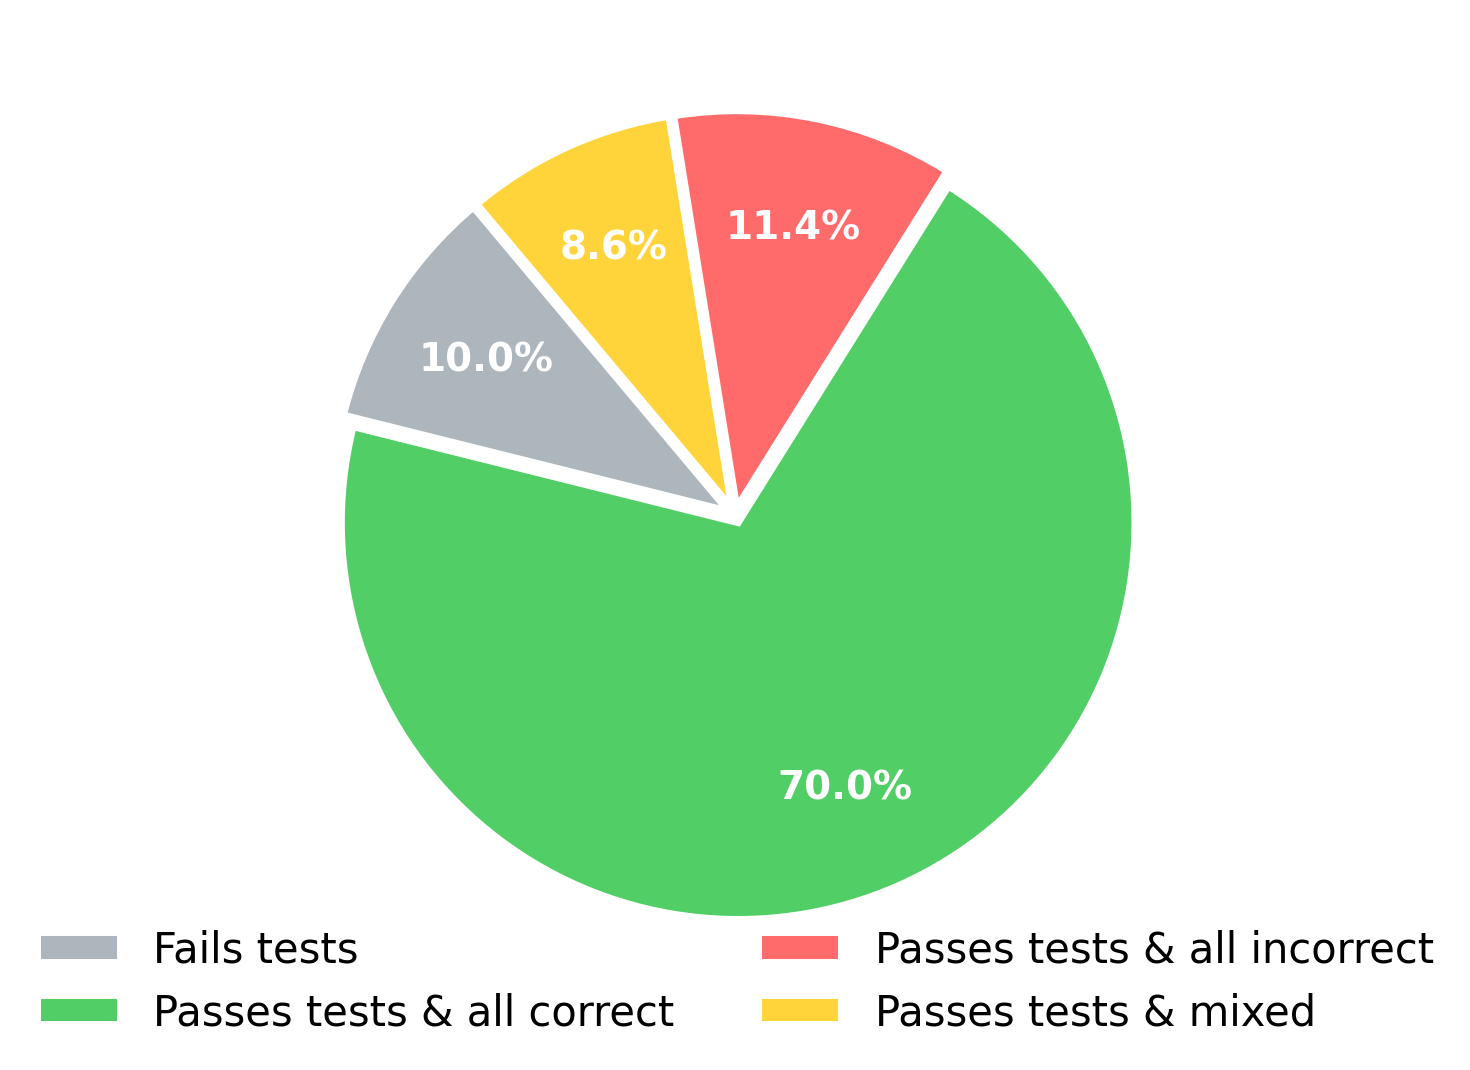
\includegraphics[width=\linewidth]{figures/branch_a2_pass_at_k.png}
  \caption{Unit-test reward (Branch A). Of 70 problems, $70.0\%$ pass the generated tests and are also judged correct against the gold-standard Verus specification. The remaining $20.0\%$ pass the tests despite being incorrect ($11.4\%$ all incorrect, $8.6\%$ a mix of correct and incorrect across the $5$ samples) -- these are reward hacks. The final $10.0\%$ fail the tests outright.}
  \label{fig:results:branch-a}
\end{subfigure}
\hfill
\begin{subfigure}[t]{0.48\textwidth}
  \centering
  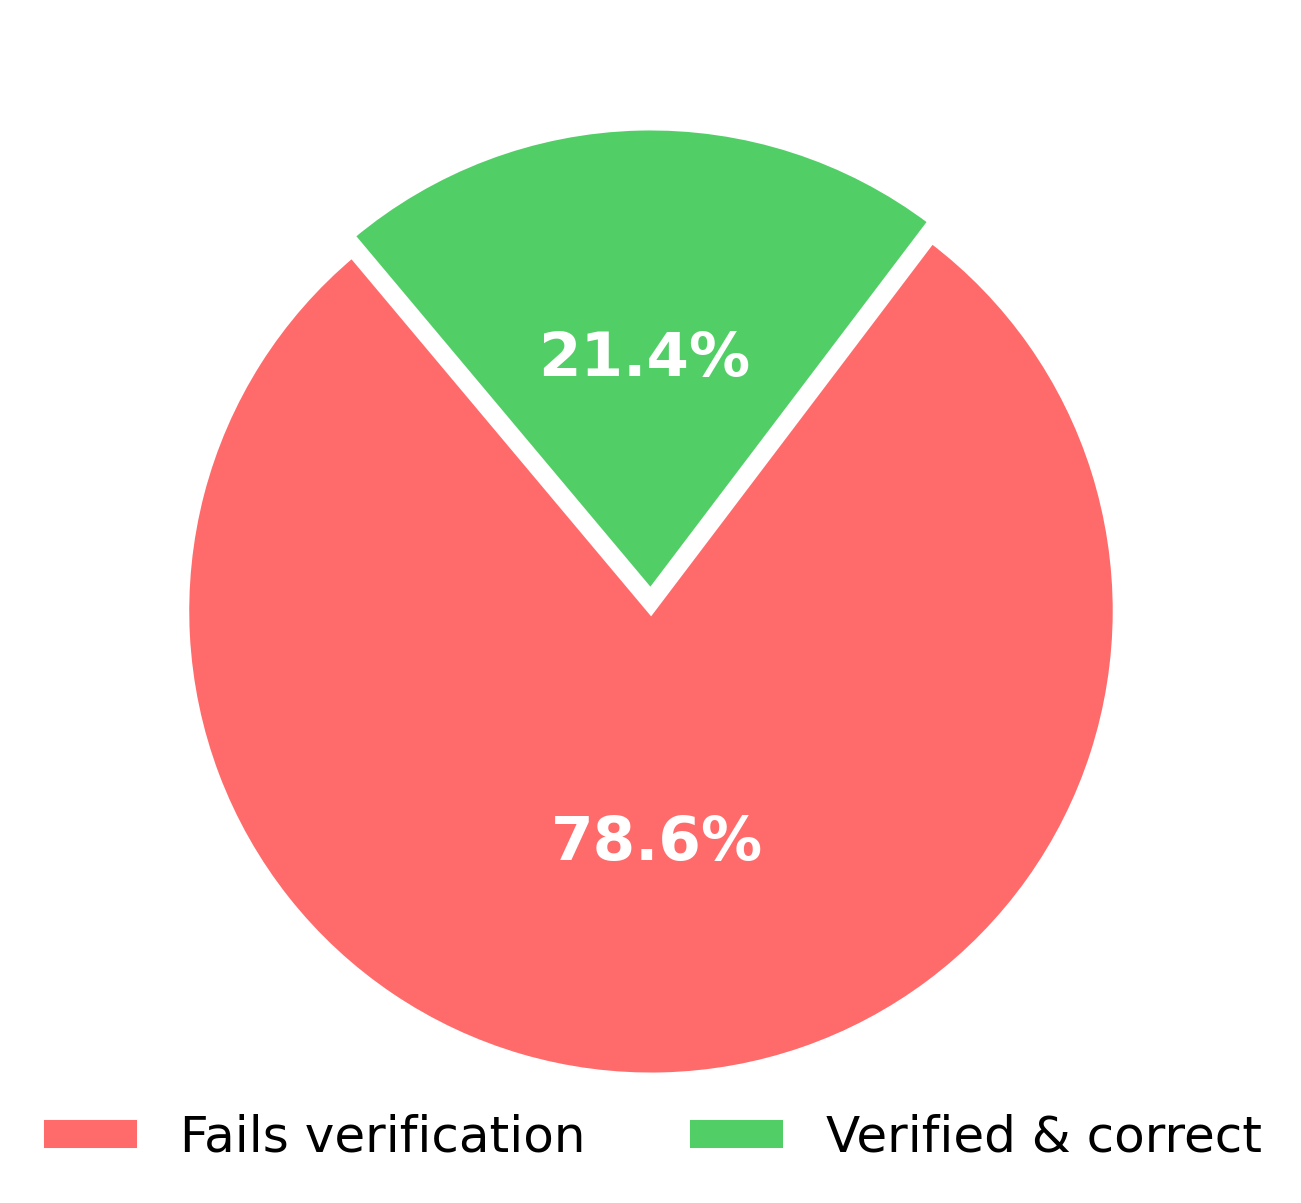
\includegraphics[width=\linewidth]{figures/branch_b_pass_at_k.png}
  \caption{Formal-spec reward (Branch B). Of 70 problems, $21.4\%$ are verified by Verus against the generated specification and judged correct against the gold-standard. The remaining $78.6\%$ fail verification. Crucially, $0\%$ of samples passed verification while being incorrect: with formal specifications, the model never reward-hacked.}
  \label{fig:results:branch-b}
\end{subfigure}
\caption{Outcome breakdown across $70$ HumanEval-Verus problems with Qwen3-Coder at pass@$5$. Reward hacking (passes the in-loop reward signal but is incorrect under the gold-standard spec) accounts for $20\%$ of unit-test outcomes (left) but $0\%$ of formal-spec outcomes (right).}
\label{fig:results-pass-at-k}

\end{figure}

Under the unit-test reward (Branch A), $70.0\%$ of problems are solved
correctly, but a further $20.0\%$ pass the generated tests while being incorrect
under the gold-standard specification ($11.4\%$ where every one of the $5$
samples is wrong, plus $8.6\%$ where the $5$ samples are a mix of correct and
incorrect implementations that all satisfy the tests). The remaining $10.0\%$
fail the tests outright. We interpret the $20.0\%$ slice as reward hacking:
the model produced code that the reward signal accepts but the
specification rejects. Manual inspection confirms the typical failure
mode is hard-coding the test inputs.

Under the formal-spec reward (Branch B), $21.4\%$ of problems are verified by
Verus and judged correct against the gold-standard, and the remaining $78.6\%$
fail verification. Notably, $0\%$ of samples passed verification while being
incorrect -- the model did not reward-hack. This is the property formal
specifications are supposed to give us: when the reward signal is a
machine-checked proof of a specification, hacking the reward requires producing
a verified-but-wrong program, which the soundness of Verus rules out (modulo
under-specification, which we did not observe in practice on these problems).

\paragraph{Takeaways.}
\begin{itemize}
\item \textbf{Reward hacking is empirically much rarer with formal specifications.}
  $20.0\%$ vs.\ $0\%$ on this benchmark.
\item \textbf{Reward hacking with formal specifications is not impossible in principle.}
  An under-specification that admits incorrect programs would still be reward
  hackable; we simply did not observe one here.
\item \textbf{Unit tests still produce more \emph{correct} code overall.} Branch
  A reaches $70.0\%$ true success vs.\ $21.4\%$ for Branch B. The bottleneck for
  Branch B is not specification quality but rather the model's ability to
  produce code together with proof annotations that Verus can check; we discuss
  this trade-off further in Section~\ref{challenges}.
\end{itemize}

\as{Experiments that we want to run next: varying model, A1 vs A2, increasing few-shot, pass@k}
